\section{Concatenated, Non-partitioned}\label{secUnif} 

Our first exercise is to construct a multi-gene analysis where all genes evolve under the same process and parameters.

To begin, load in the sequences using the \cl{readDiscreteCharacterData()} function. 
{\tt \begin{snugshade*}
\begin{lstlisting}
data_cox2 = readDiscreteCharacterData("data/primates_cox2.nex")
data_cytb = readDiscreteCharacterData("data/primates_cytb.nex")
\end{lstlisting}
\end{snugshade*}}

Since the first step in this exercise is to assume a single model across genes, we need to combine the two datasets using {\tt concatenate()}

{\tt \begin{snugshade*}
\begin{lstlisting}
data = concatenate( data_cox2, data_cytb )
\end{lstlisting}
\end{snugshade*}}

Typing \cl{data} reports the dimensions of the concatenated matrix, this provides information about the alignment:


{\tt \begin{snugshade*}
\begin{lstlisting}

   DNA character matrix with 23 taxa and 1852 characters
   =====================================================
   Origination:                   primates_cox2.nex
   Number of taxa:                23
   Number of included taxa:       23
   Number of characters:          1852
   Number of included characters: 1852
   Datatype:                      DNA

\end{lstlisting}
\end{snugshade*}}

For later use, we will store the taxon labels (\cl{names}), the number of species (\cl{n\_species}), the number of internal branches (\cl{n\_branches}), and the number of sites (\cl{n\_sites}).

{\tt \begin{snugshade*}
\begin{lstlisting}
names <- data.names()
n_species <- data.ntaxa()
n_branches <- 2 * n_species - 3
n_sites <- data.nchar()
\end{lstlisting}
\end{snugshade*}}

Additionally, we will create some move and monitor index variables to create our move and monitor vectors.

{\tt \begin{snugshade*}
\begin{lstlisting}
mvi <- 1
mni <- 1
\end{lstlisting}
\end{snugshade*}}

Now we can proceed with building our GTR$+\Gamma$ model.
First, we will define and specify a prior on the exchangeability rates of the GTR model

{\tt \begin{snugshade*}
\begin{lstlisting}
er_prior <- v(1,1,1,1,1,1) 
er ~ dnDirichlet( er_prior )
\end{lstlisting}
\end{snugshade*}}

and assign its move

{\tt \begin{snugshade*}
\begin{lstlisting}
moves[mvi++] = mvSimplexElementScale(er, alpha=10, tune=true, weight=15) 
\end{lstlisting}
\end{snugshade*}}

We can use the same type of distribution as a prior on the 4 stationary frequencies ($\pi_A, \pi_C, \pi_G, \pi_T$) since these parameters also represent proportions. 
Specify a flat Dirichlet prior density on the base frequencies:
{\tt \begin{snugshade*}
\begin{lstlisting}
sf_prior <- v(1,1,1,1) 
sf ~ dnDirichlet( sf_prior )
\end{lstlisting}
\end{snugshade*}}

The node \cl{sf} represents the $\pi$ node in Figure \ref{gtrgmfig}.
Now add the simplex scale move on the stationary frequencies to the moves vector

{\tt \small \begin{snugshade*}
\begin{lstlisting}
moves[mvi++] = mvSimplexElementScale(sf, alpha=10, tune=true, weight=15) 
\end{lstlisting}
\end{snugshade*}}

We can finish setting up this part of the model by creating a deterministic node for the GTR rate matrix \cl{Q}. 
The \cl{fnGTR()} function takes a set of exchangeability rates and a set of base frequencies to compute the rate matrix used when calculating the likelihood of our model.
{\tt \begin{snugshade*}
\begin{lstlisting}
Q := fnGTR(er,sf)
\end{lstlisting}
\end{snugshade*}}


We will also assume that the substitution rates vary among sites according to a gamma distribution, which has two parameters: the shape parameter, $\alpha$, and the rate parameter, $\beta$. 
In order that we can interpret the branch lengths as the expected number of substitutions per site, this model assumes that the mean site rate is equal to 1.
%Consequently, we wish to specify a gamma distribution with a mean of 1.
The mean of the gamma is equal to $\alpha/\beta$, so a mean-one gamma is specified by setting the two parameters to be equal, $\alpha=\beta$.
Therefore, we need only consider the single shape parameter, $\alpha$ \citep{yang94a}. 
The degree of among-site substitution rate variation (ASRV) is inversely proportional to the value of the shape parameter---as the value of $\alpha$-shape parameter increases, the gamma distribution increasingly resembles a normal distribution with decreasing variance, which corresponds to decreasing levels of ASRV (Figure \ref{asrhGammaFig}).
If $\alpha = 1$, then the gamma distribution collapses to an exponential distribution with a rate parameter equal to $\beta$.
By contrast, when the value of the $\alpha$-shape parameter is $< 1$, the gamma distribution assumes a concave distribution that places most of the prior density on low rates but allows some prior mass on sites with very high rates, which corresponds to high levels of ASRV (Figure \ref{asrhGammaFig}).

\begin{figure}[h]
\centering
\fbox{\includegraphics[width=2.5in,angle=-90]{\ResourcePath figures/asrh_gamma.eps}}
\caption{\small The probability density of mean-one gamma-distributed rates under different shape parameters.}
\label{asrhGammaFig}
\end{figure}


Alternatively, we might not have good prior knowledge about the variance in site rates, thus we can place an uninformative, or diffuse prior on the shape parameter.
For this analysis, we will use an exponential distribution with a rate parameter, \cl{shape\_prior}, equal to \cl{0.05}.
Under an exponential prior, we are placing non-zero probability on values of $\alpha$ ranging from 0 to $\infty$. 
The rate parameter, often denoted $\lambda$, of an exponential distribution controls both the mean and variance of this prior such that the expected (or mean) value of $\alpha$ is:
$\mathbb{E}[\alpha] = \frac{1}{\lambda}.$
Thus, if we set $\lambda=0.05$, then $\mathbb{E}[\alpha] = 20$.

Create a constant node called \cl{shape\_prior} for the rate parameter of the exponential prior on the gamma-shape parameter
{\tt\begin{snugshade*}
\begin{lstlisting}
alpha_prior_min <- 0.1
alpha_prior_max <- 50.0
\end{lstlisting}
\end{snugshade*}}

Then create a stochastic node called \cl{shape} to represent the $\alpha$ node in Figure \ref{gtrgmfig}, with an exponential density as a prior:
{\tt\begin{snugshade*}
\begin{lstlisting}
alpha ~ dnUnif( alpha_prior_min, alpha_prior_max )
\end{lstlisting}
\end{snugshade*}}

The way the ASRV model is implemented involves discretizing the mean-one gamma distribution into a set number of rate categories. Thus, we can analytically marginalize over the uncertainty in the rate at each site. To do this, we need a deterministic node that is a vector of rates calculated from the gamma distribution and the number of rate categories. The \cl{fnDiscretizeGamma()} function returns this deterministic node and takes three arguments: the shape and rate of the gamma distribution and the number of categories. Since we want to discretize a mean-one gamma distribution, we can pass in \cl{shape} for both the shape and rate.

Initialize the \cl{gamma\_rates} deterministic node vector using the  \cl{fnDiscretizeGamma()} function with \cl{4} bins:
{\tt \begin{snugshade*}
\begin{lstlisting}
norm_gamma_rates := fnDiscretizeGamma( alpha, alpha, 4, false )
\end{lstlisting}
\end{snugshade*}}

The random variable that controls the rate variation is the stochastic node \cl{shape}. This variable is a single, real positive value (\cl{RevType = RealPos}). 
We will apply a simple scale move to this parameter.
The scale move's tuning parameter is called \cl{lambda} and this value dictates the size of the proposal.
{\tt \begin{snugshade*}
\begin{lstlisting}
moves[mvi++] = mvScale(alpha, lambda=0.1, tune=false, weight=4.0)
\end{lstlisting}
\end{snugshade*}}

Invariant sites (sites that remain fixed throughout their evolutionary history) may be seen as an extreme case of among-site rate variation.
In contrast to $+ \Gamma$ models, the $+I$ model allows site some probability of having substitution rate equal to zero.
Only if a site has an invariant pattern (they are all are equal) there is some non-zero probability of the site being classified as invariant.
(Seeing an invariant site pattern does not necessarily indicate the site evolved according to an invariant process: there is some probability of some substitution later being erased through a character reversion, which must be accounted for in the $+I$ model.)

Here, we give the probability of a site being invariant with {\tt pinvar}
{\tt \begin{snugshade*}
\begin{lstlisting}
pinvar ~ dnBeta(1,1)
moves[mvi++] = mvScale(pinvar, lambda=0.1, tune=false, weight=2.0)
moves[mvi++] = mvSlide(pinvar, delta=10.0, tune=false, weight=2.0)
\end{lstlisting}
\end{snugshade*}}

Note, if the $+\Gamma$ model allows for one rate category to take a very small value, it approximates the zero-rate value for the $+I$ model.
This means when invariant site patterns are present, the $+\Gamma$ and $+I$ models vie to explain the same underlying evolutionary process of some sites evolving at a zero or near-zero rate.

The tree topology and branch lengths are also stochastic nodes in our model. 
In Figure \ref{gtrgmfig}, the tree topology is denoted $\Psi$ and the length of the branch leading to node $i$ is $\nu_i$.

We will assume the topology and divergence times are distributed by a birth-death process called \cl{dnBDP()} in RevBayes.
First, we will define the distribution's speciation rate, {\tt lambda}, and an extinction rate {\tt mu}

{\tt \begin{snugshade*}
\begin{lstlisting}
speciation ~ dnExponential(10.0)
extinction ~ dnExponential(10.0)
moves[mvi++] = mvScale(speciation, weight=5)
moves[mvi++] = mvScale(extinction, weight=5)
\end{lstlisting}
\end{snugshade*}}

Since we know our analysis contains only 23 of 270 known primate species, we may inform the birth-death process only a portion of taxa were sampled.
Failing to do so artificially inflates the extinction rate.

{\tt \begin{snugshade*}
\begin{lstlisting}
sampling_fraction <- 23. / 270 # 23 out of the ~ 270 primate species
\end{lstlisting}
\end{snugshade*}}

To simplify the analysis, we assume the tree height is known to be 75, although in practice this quantity should be treated as a free parameter to estimate.

{\tt \begin{snugshade*}
\begin{lstlisting}
psi ~ dnBDP(lambda=speciation, mu=extinction, rho=sampling_fraction, rootAge=75, names=names)
\end{lstlisting}
\end{snugshade*}}

Finally, we will provide moves so the MCMC may explore the space of tree topologies ({\tt mvNNI} and {\tt mvFNPR}, the nearest-neighbor interchange and fixed-node-height-prune-regraft proposals, resp.) and the space of divergence times ({\tt mvNodeTimeSlideUniform}).

{\tt \begin{snugshade*}
\begin{lstlisting}
moves[mvi++] = mvNNI(psi, weight=10.0)
moves[mvi++] = mvFNPR(psi, weight=5.0)
moves[mvi++] = mvNodeTimeSlideUniform(psi, weight=10.0)
\end{lstlisting}
\end{snugshade*}}

Also for simplicity, we assume a global molecular clock

{\tt \small \begin{snugshade*}
\begin{lstlisting}
clock ~ dnExponential(10.0)
moves[mvi++] = mvScale(clock, lambda=1, tune=true, weight=3.0)
\end{lstlisting}
\end{snugshade*}}

We now have all the parameters needed to model the phylogenetic molecular substitution process

{\tt \begin{snugshade*}
\begin{lstlisting}
phyloSeq ~ dnPhyloCTMC(tree=psi, Q=Q, branchRates=clock, siteRates=norm_gamma_rates, pInv=pinvar, type="DNA")
\end{lstlisting}
\end{snugshade*}}

To compute the likelihood, we condition the process on the data observed at the tips of the tree

{\tt \begin{snugshade*}
\begin{lstlisting}
phyloSeq.clamp(data)
\end{lstlisting}
\end{snugshade*}}

Since the model is now specified, we wrap the components in a {\tt Model} object.

{\tt \begin{snugshade*}
\begin{lstlisting}
mymodel = model(Q)
\end{lstlisting}
\end{snugshade*}}

For our MCMC analysis we need to set up a vector of \textit{monitors} to save the states of our Markov chain. 
The monitor functions are all called \cl{mn*}, where \cl{*} is the wildcard representing the monitor type.
First, we will initialize the model monitor using the \cl{mnModel} function. This creates a new monitor variable that will output the states for all model parameters when passed into a MCMC function. 
{\tt \begin{snugshade*}
\begin{lstlisting}
monitors[mni++] = mnModel(filename="output/PS0.params.txt",printgen=10)
\end{lstlisting}
\end{snugshade*}}

The \cl{mnFile} monitor will record the states for only the parameters passed in as arguments. We use this monitor to specify the output for our sampled trees and branch lengths.

{\tt \begin{snugshade*}
\begin{lstlisting}
monitors[mni++] = mnFile(psi, filename="output/PS0.tre", printgen=100)
\end{lstlisting}
\end{snugshade*}}

Finally, create a screen monitor that will report the states of specified variables to the screen with \cl{mnScreen}:
{\tt \begin{snugshade*}
\begin{lstlisting}
monitors[mni++] = mnScreen(er, sf, alpha, norm_gamma_rates, pinvar, speciation, extinction, clock, printgen=100)
\end{lstlisting}
\end{snugshade*}}

With a fully specified model, a set of monitors, and a set of moves, we can now set up the MCMC algorithm that will sample parameter values in proportion to their posterior probability. The \cl{mcmc()} function will create our MCMC object:
{\tt \begin{snugshade*}
\begin{lstlisting}
mymcmc = mcmc(mymodel, monitors, moves)
\end{lstlisting}
\end{snugshade*}}

We can run the \cl{.burnin()} member function if we wish to pre-run the chain and discard the initial states. 
{\tt \begin{snugshade*}
\begin{lstlisting}
mymcmc.burnin(generations=10000,tuningInterval=100)
\end{lstlisting}
\end{snugshade*}}


Now, run the MCMC:
{\tt \begin{snugshade*}
\begin{lstlisting}
mymcmc.run(generations=30000)
\end{lstlisting}
\end{snugshade*}}

When the analysis is complete, you will have the monitor files in your output directory.

Methods for visualizing the marginal densities of parameter values are not currently available in \RevBayes. Thus, it is important to use programs like Tracer \citep{rambaut09} to evaluate mixing and non-convergence. (RevBayes does, however, have a tool for convergence assessment called \cl{beca}.)

\RevBayes~can also summarize the tree samples by reading in the tree-trace file:
{\tt \begin{snugshade*}
\begin{lstlisting}
treetrace = readTreeTrace("output/model_PS0.tre")
treetrace.summarize()
\end{lstlisting}
\end{snugshade*}}


The \cl{mapTree()} function will summarize the tree samples and write the maximum a posteriori tree to file:
{\tt \begin{snugshade*}
\begin{lstlisting}
mapTree(treetrace,"output/model_PS0_map.tre")
\end{lstlisting}
\end{snugshade*}}

This completes the uniform partition analysis.
The next two sections will implement more complex partitioning schemes in a similar manner.
